\documentclass[11pt,a4paper]{article}

\usepackage[T1]{fontenc}
\usepackage{lmodern}
\usepackage{microtype}
\usepackage[margin=2.5cm]{geometry}

\usepackage{amsmath,amssymb}
\usepackage{booktabs}
\usepackage{array}
\usepackage{siunitx}
\sisetup{group-separator={,},group-minimum-digits=4}
\usepackage{tikz}
\usetikzlibrary{positioning,arrows.meta,calc}
\usepackage{listings}
\usepackage[hidelinks,colorlinks=true,linkcolor=black,citecolor=black,urlcolor=blue!60!black]{hyperref}
\usepackage{url}
\usepackage{enumitem}
\usepackage{cleveref}
\setlist{nosep,leftmargin=1.5em}

\lstset{
  basicstyle=\small\ttfamily,
  keywordstyle=\bfseries,
  breaklines=true,
  frame=single,
  framesep=4pt,
  xleftmargin=4pt,
  xrightmargin=4pt,
  aboveskip=6pt,
  belowskip=6pt,
  columns=fullflexible,
  keepspaces=true,
  morekeywords={iter,const,let,import,from,yield,function,for,of,if,return,
    break,export,type,number,string,boolean,void}
}

% ============================================================
\title{iterflow: Composable Streaming Statistics for JavaScript}

\author{
  Gaurav Singh\\
  Mathscapes Research\\
  \texttt{gv-sh@outlook.com}
}

\date{February 2026}

\begin{document}
\maketitle

% ============================================================
\begin{abstract}
We present \texttt{iterflow}, a zero-dependency JavaScript library that integrates online statistical algorithms into lazy iterator pipelines. ES2025 Iterator Helpers provide lazy transforms but no statistics; libraries like \texttt{@stdlib/stats/incr} provide streaming accumulators but not as composable pipeline stages. \texttt{iterflow} bridges this gap: Welford's variance, EWMA, streaming Pearson correlation, z-score anomaly detection, and monotonic deque windowed extrema are implemented as chainable pipeline stages that compose with \texttt{map}, \texttt{filter}, \texttt{window}, and \texttt{take} while preserving lazy evaluation and $O(1)$ memory per stage. Benchmarks on synthetic workloads show a $296\times$ throughput improvement over eager array pipelines with early termination at $N{=}10^6$, and a $780\times$ improvement for streaming versus recomputed correlation at $N{=}10^4$. For standalone single-statistic computation, the generator-based design incurs $3$--$5\times$ overhead relative to hand-written loops.

\medskip
\noindent\textbf{Keywords:} streaming algorithms, iterator pipelines, online statistics, JavaScript, lazy evaluation
\end{abstract}

% ============================================================
\section{Introduction}

A recurring pattern in server-side JavaScript is the need to compute running statistics over data too large or too incremental to materialise: monitoring dashboards processing millions of metrics, log analyzers scanning multi-gigabyte files, and sensor pipelines producing unbounded streams. Two capabilities are required. First, \emph{lazy evaluation}: elements should be processed on demand, pipelines should terminate early, and intermediate arrays should not be allocated. Second, \emph{streaming statistics}: mean, variance, correlation, and anomaly scores should be computable in a single pass with bounded memory.

JavaScript now offers partial solutions to each. ES2025 Iterator Helpers~\cite{tc39iterators} added lazy \texttt{map}, \texttt{filter}, \texttt{take}, and \texttt{flatMap} to the iterator protocol, but no statistical operations; computing a windowed variance still requires collecting into an array. Conversely, \texttt{@stdlib/stats/incr}~\cite{stdlib} provides high-quality standalone streaming accumulators---incremental mean, variance, covariance---but these are imperative objects, not composable pipeline stages. A workflow like ``filter valid readings $\to$ sliding window $\to$ compute variance $\to$ threshold $\to$ take first 100'' requires the user to manually iterate, manage circular buffers, feed each value into an accumulator, and implement early termination logic.

\texttt{iterflow} unifies lazy pipeline composition with streaming statistical algorithms. Its contribution is a \emph{composition model} in which online algorithms are first-class pipeline stages: a pipeline \texttt{filter}$\to$\texttt{window}$\to$\texttt{streamingVariance}$\to$\texttt{take} is expressed as a single chained expression, executes in constant memory, and terminates the moment the \texttt{take} count is satisfied.

The library is published as \texttt{@mathscapes/iterflow} on npm under the MIT license. It has zero runtime dependencies, full TypeScript type inference, and dual ESM/CJS builds. Source code and benchmarks are available at \url{https://github.com/mathscapes/iterflow}. DOI: \href{https://doi.org/10.5281/zenodo.18610143}{10.5281/zenodo.18610143}.

% ============================================================
\section{Related Work}
\label{sec:related}

\begin{table}[t]
\centering
\caption{Capability matrix for JavaScript data processing libraries.}
\label{tab:comparison}
\small
\begin{tabular}{@{} l @{\hspace{6pt}} c @{\hspace{6pt}} c @{\hspace{6pt}} c @{\hspace{6pt}} c @{\hspace{6pt}} c @{}}
\toprule
& \texttt{iterflow}
& \begin{tabular}[c]{@{}c@{}}ES2025\\Iter.\end{tabular}
& \texttt{@stdlib}
& RxJS
& \begin{tabular}[c]{@{}c@{}}simple-\\statistics\end{tabular} \\
\midrule
Lazy evaluation      & $\bullet$ & $\bullet$ &           & $\bullet$ &           \\
Streaming statistics  & $\bullet$ &           & $\bullet$ &           &           \\
Pipeline composition  & $\bullet$ & $\bullet$ &           & $\bullet$ &           \\
Synchronous batch     & $\bullet$ & $\bullet$ & $\bullet$ &           & $\bullet$ \\
Windowed aggregation  & $\bullet$ &           &           & $\bullet$ &           \\
Early termination     & $\bullet$ & $\bullet$ &           &           &           \\
Zero dependencies     & $\bullet$ & native    &           &           & $\bullet$ \\
\bottomrule
\end{tabular}
\end{table}

\Cref{tab:comparison} summarises the landscape. No existing JavaScript library combines lazy pipeline composition with streaming statistics.

\textbf{ES2025 Iterator Helpers}~\cite{tc39iterators} reached Stage 4 in 2025 and provide \texttt{.map()}, \texttt{.filter()}, \texttt{.take()}, \texttt{.drop()}, and \texttt{.flatMap()} on the iterator prototype. \texttt{iterflow} mirrors this API surface but extends it with windowing, chunking, and statistical operations. When transforms alone suffice, native helpers are preferable; \texttt{iterflow}'s value appears when statistical computation must compose within the pipeline.

\textbf{\texttt{@stdlib/stats/incr}}~\cite{stdlib} provides streaming accumulators with careful numerical treatment. However, the accumulators are standalone objects: composing ``filter $\to$ sliding window $\to$ variance $\to$ anomaly detection'' requires imperative loops, manual buffer management, and bespoke early-termination logic. The composition burden falls entirely on the user.

\textbf{RxJS}~\cite{rxjs} targets asynchronous reactive streams with concepts (Observables, Schedulers, backpressure) designed for event-driven I/O. It lacks built-in streaming statistical operators and introduces abstraction overhead unnecessary for synchronous batch analysis.

\textbf{simple-statistics}~\cite{simplestatistics} provides a broad set of statistical functions operating on materialised arrays. It cannot process infinite or very large streams and does not support early termination.

% ============================================================
\section{Design}
\label{sec:design}

\subsection{Pipeline composition via generators}

The core abstraction is \texttt{Iterflow<T>}, a lightweight wrapper around JavaScript's iterable protocol. Each transform method---\texttt{map}, \texttt{filter}, \texttt{window}, \texttt{streamingVariance}, etc.---returns a new \texttt{Iterflow} backed by a generator function that lazily pulls values from the upstream source. No computation occurs until a terminal method (\texttt{toArray}, \texttt{reduce}, \texttt{first}, etc.) drives the iteration. \Cref{fig:pipeline} illustrates the architecture.

\begin{figure}[t]
\centering
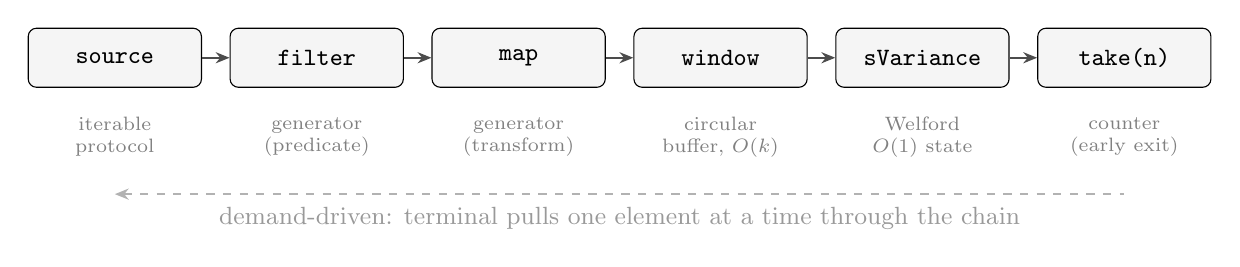
\begin{tikzpicture}[
  stage/.style={
    draw, rounded corners=3pt,
    minimum height=0.75cm, minimum width=2.2cm,
    font=\small\ttfamily, fill=black!4, inner sep=4pt
  },
  impl/.style={font=\scriptsize, text=black!50, align=center},
  arr/.style={-{Stealth[length=5pt,width=4pt]}, thick, black!70},
  node distance=0.5cm and 0.35cm
]

  % Top row: pipeline stages
  \node[stage] (src)    {source};
  \node[stage, right=of src]    (filt)   {filter};
  \node[stage, right=of filt]   (mp)     {map};
  \node[stage, right=of mp]     (win)    {window};
  \node[stage, right=of win]    (svar)   {sVariance};
  \node[stage, right=of svar]   (take)   {take(n)};

  % Arrows between stages
  \draw[arr] (src)  -- (filt);
  \draw[arr] (filt) -- (mp);
  \draw[arr] (mp)   -- (win);
  \draw[arr] (win)  -- (svar);
  \draw[arr] (svar) -- (take);

  % Implementation labels below
  \node[impl, below=0.25cm of src]  {iterable\\protocol};
  \node[impl, below=0.25cm of filt] {generator\\(predicate)};
  \node[impl, below=0.25cm of mp]   {generator\\(transform)};
  \node[impl, below=0.25cm of win]  {circular\\buffer, $O(k)$};
  \node[impl, below=0.25cm of svar] {Welford\\$O(1)$ state};
  \node[impl, below=0.25cm of take] {counter\\(early exit)};

  % Pull arrow
  \draw[{Stealth[length=5pt,width=4pt]}-, thick, dashed, black!30]
    ([yshift=-1.35cm]src.south) -- ([yshift=-1.35cm]take.south)
    node[midway, below=1pt, font=\small, text=black!40]
    {demand-driven: terminal pulls one element at a time through the chain};

\end{tikzpicture}
\caption{Architecture of a six-stage pipeline. Each stage is a generator function; the terminal (\texttt{take}) pulls elements through the chain one at a time. No intermediate arrays are allocated between stages. Stages maintain only their local state (e.g., circular buffer for \texttt{window}, three scalars for Welford's algorithm in \texttt{sVariance}).}
\label{fig:pipeline}
\end{figure}

This design yields two properties. First, memory usage is $O(1)$ per stateless stage and $O(k)$ per windowed stage, independent of input size. Second, early termination propagates automatically: when \texttt{take(n)} stops pulling, upstream generators are never resumed, and unprocessed elements are never touched.

\subsection{Type constraints}

Statistical methods are constrained to \texttt{Iterflow<number>} via TypeScript method overloading. Calling \texttt{.sum()} on \texttt{Iterflow<string>} is a compile-time error, ensuring that streaming statistical stages receive numeric input without runtime type checks on the hot path.

% ============================================================
\section{Streaming Algorithms}
\label{sec:algorithms}

\Cref{tab:complexity} summarises the operations and their asymptotic complexity. All streaming transforms maintain bounded state and consume elements in a single pass.

\begin{table}[t]
\centering
\caption{Time and space complexity of streaming operations. $n$ = elements processed, $k$ = window size.}
\label{tab:complexity}
\small
\begin{tabular}{@{} l l l l @{}}
\toprule
Operation & Time & Space & Reference \\
\midrule
\texttt{streamingMean}        & $O(n)$         & $O(1)$ & \cref{eq:mean} \\
\texttt{streamingVariance}    & $O(n)$         & $O(1)$ & Welford~\cite{welford1962} \\
\texttt{ewma($\alpha$)}      & $O(n)$         & $O(1)$ & Hunter~\cite{hunter1986} \\
\texttt{streamingCovariance}  & $O(n)$         & $O(1)$ & Chan et al.~\cite{chan1982} \\
\texttt{streamingCorrelation} & $O(n)$         & $O(1)$ & Chan et al.~\cite{chan1982} \\
\texttt{streamingZScore}      & $O(n)$         & $O(1)$ & \cref{eq:zscore} \\
\texttt{windowedMin/Max}      & $O(n)$         & $O(k)$ & Lemire~\cite{lemire2006} \\
\texttt{window($k$)}         & $O(n)$         & $O(k)$ & circular buffer \\
\texttt{variance} (terminal)  & $O(n)$         & $O(1)$ & Welford~\cite{welford1962} \\
\texttt{median} (terminal)    & $O(n)$ avg.    & $O(n)$ & Hoare~\cite{hoare1961} \\
\bottomrule
\end{tabular}
\end{table}

\textbf{Online mean and variance.}
Streaming variance uses Welford's algorithm~\cite{welford1962}, which avoids the catastrophic cancellation inherent in na\"{i}ve two-pass or sum-of-squares formulations~\cite{higham2002}. Given observations $x_1, \ldots, x_n$, the algorithm maintains a running mean $M_k$ and aggregate squared deviation $S_k$:
\begin{align}
  M_k &= M_{k-1} + \frac{x_k - M_{k-1}}{k} \label{eq:mean} \\[4pt]
  S_k &= S_{k-1} + (x_k - M_{k-1})(x_k - M_k) \label{eq:welford}
\end{align}
Population variance at step $k$ is $\sigma^2_k = S_k / k$. The entire state consists of three scalars $(k, M_k, S_k)$.

\textbf{Exponentially weighted moving average.}
EWMA~\cite{hunter1986} computes a smoothed estimate that emphasises recent observations:
\begin{equation}
  \text{EWMA}_t = \alpha \cdot x_t + (1 - \alpha) \cdot \text{EWMA}_{t-1}, \quad \alpha \in (0, 1]
  \label{eq:ewma}
\end{equation}
with $\text{EWMA}_0 = x_0$. The decay factor $\alpha$ controls responsiveness. State: one scalar.

\textbf{Streaming covariance and Pearson correlation.}
The bivariate extension of Welford's method~\cite{chan1982} computes covariance and correlation from paired streams $\{(x_i, y_i)\}$ in a single pass, maintaining means $\bar{x}_k, \bar{y}_k$, second moments $M_{2x,k}, M_{2y,k}$, and co-moment $C_{xy,k}$:
\begin{align}
  C_{xy,k} &= C_{xy,k-1} + (x_k - \bar{x}_{k-1})(y_k - \bar{y}_k) \\[4pt]
  r_k &= \frac{C_{xy,k}}{\sqrt{M_{2x,k} \cdot M_{2y,k}}} \label{eq:corr}
\end{align}
State: six scalars. $r_k$ yields the Pearson correlation coefficient at each step.

\textbf{Streaming z-score.}
Anomaly detection via z-score uses the mean and standard deviation accumulated from \emph{prior} observations:
\begin{equation}
  z_k = \frac{x_k - M_{k-1}}{\sqrt{S_{k-1} / (k-1)}} \label{eq:zscore}
\end{equation}
This pre-observation convention prevents the current value from influencing its own score. The first two elements yield NaN (insufficient data for a meaningful standard deviation).

\textbf{Monotonic deque windowed extrema.}
Sliding-window minimum and maximum use monotonic deques~\cite{lemire2006} to maintain the current extremum in $O(1)$ amortised time per element. Each element enters and leaves the deque at most once, giving $O(n)$ total work with $O(k)$ space. This avoids the $O(nk)$ cost of na\"{i}ve rescanning.

\textbf{Circular buffer windowing.}
The \texttt{window(k)} transform writes each element at position $i \bmod k$ in a pre-allocated array, avoiding the $O(k)$ per-element cost of \texttt{shift()}-based na\"{i}ve sliding windows.

\textbf{Quickselect median.}
The terminal \texttt{median()} uses Hoare's quickselect~\cite{hoare1961} for $O(n)$ average-case selection, avoiding the $O(n \log n)$ cost of a full sort. NaN values are filtered before selection.

% ============================================================
\section{Evaluation}
\label{sec:eval}

We evaluate \texttt{iterflow} on four benchmark suites using Tinybench on Node.js v22 (ARM64 Linux). All benchmarks are included in the repository and are reproducible via \texttt{node --import tsx benchmarks/*.bench.ts}. Data is synthetically generated; results report mean throughput over the default Tinybench iteration count.

\subsection{Lazy evaluation with early termination}

The primary motivation for \texttt{iterflow} is pipelines that terminate early on large inputs. \Cref{tab:lazy} measures a filter$\to$map$\to$take(1000) pipeline as input size $N$ varies.

\begin{table}[t]
\centering
\caption{Filter-map-take(1000) pipeline throughput (ops/s). \texttt{iterflow} uses lazy generators; ``Native array'' uses \texttt{.filter().map().slice()}. Throughput RME below 1\% for all measurements.}
\label{tab:lazy}
\small
\begin{tabular}{@{} r S[table-format=5.0] S[table-format=7.0] r @{}}
\toprule
{$N$} & {\texttt{iterflow}} & {Native array} & {Ratio} \\
\midrule
{$10^2$}   & 69268  & 1538911 & {$0.05\times$} \\
{$10^3$}   & 9812   & 143443  & {$0.07\times$} \\
{$10^4$}   & 7859   & 13380   & {$0.59\times$} \\
{$10^5$}   & 7917   & 434     & {$18.2\times$} \\
{$10^6$}   & 7818   & 26      & {$\mathbf{296\times}$} \\
\bottomrule
\end{tabular}
\end{table}

The key observation is that \texttt{iterflow}'s throughput is effectively constant across $N$ (${\sim}8{,}000$ ops/s), because only ${\sim}1{,}000$ elements traverse the full pipeline regardless of input size. Native array methods materialise the entire filtered and mapped result before slicing, degrading linearly. The crossover occurs between $N = 10^4$ and $N = 10^5$.

For small inputs ($N < 10^3$), the generator-based pipeline is slower due to per-element overhead from \texttt{yield}/\texttt{next()} dispatch. This is the expected trade-off: generators have higher constant factors than tight array loops, but their $O(1)$ work for early termination dominates at scale.

\subsection{Streaming versus recomputed correlation}

\Cref{tab:corr} compares \texttt{streamingCorrelation} (single-pass, $O(n)$) against a two-pass baseline that recomputes Pearson $r$ from scratch at each step ($O(n^2)$ total).

\begin{table}[t]
\small
\begin{minipage}[t]{0.48\linewidth}
\centering
\caption{Streaming Pearson correlation over $N = 10{,}000$ paired observations.}
\label{tab:corr}
\begin{tabular}{@{} l S[table-format=3.2] S[table-format=4.1] @{}}
\toprule
{Method} & {Lat.\ (ms)} & {Tput.\ (ops/s)} \\
\midrule
{{\texttt{iterflow}} (1-pass)} & 0.66 & 1514 \\
{Two-pass recompute}           & 518  & 1.9 \\
\midrule
{Ratio} & \multicolumn{2}{r}{$\mathbf{780\times}$} \\
\bottomrule
\end{tabular}
\end{minipage}%
\hfill
\begin{minipage}[t]{0.48\linewidth}
\centering
\caption{Standalone statistical terminals, $N = 10^5$.}
\label{tab:stats}
\begin{tabular}{@{} l S[table-format=4.0] S[table-format=4.0] r @{}}
\toprule
{Terminal} & {\texttt{iterflow}} & {Na\"{i}ve} & {Ratio} \\
\midrule
Mean     & 8022 & 1444 & {$5.6\times$} \\
Variance & 1815 & 691  & {$2.6\times$} \\
\bottomrule
\end{tabular}
\end{minipage}
\end{table}

The improvement is algorithmic, not implementation-specific: $O(n)$ versus $O(n^2)$ total work. Any single-pass streaming implementation would show a similar advantage over the two-pass approach.

\subsection{Statistical terminals}

\Cref{tab:stats} compares \texttt{iterflow}'s terminal statistics against na\"{i}ve JavaScript implementations on a full dataset with no pipeline composition overhead. Na\"{i}ve mean uses \texttt{Array.reduce}; na\"{i}ve variance uses two-pass sum-of-squares. Throughput RME below 1\% for all measurements.

\texttt{iterflow}'s variance benefits from Welford's single-pass formulation, which avoids the second pass that the na\"{i}ve implementation requires. The mean improvement arises from a plain \texttt{for-of} loop avoiding the per-element callback overhead of \texttt{Array.prototype.reduce}.

\subsection{Generator overhead}

For operations where \texttt{iterflow} wraps a single algorithm with no pipeline composition benefit, the generator machinery adds measurable overhead. EWMA at $N = 10^5$: \texttt{iterflow} achieves 213 ops/s versus 951 ops/s for a hand-written loop ($4.5\times$ overhead). Streaming z-score: 175 ops/s versus 594 ops/s ($3.4\times$). This overhead is the per-element cost of the generator protocol (\texttt{yield}/\texttt{next()} plus closure allocation) and is inherent to the pipeline abstraction. It is fixed per element and amortised in multi-stage pipelines where the alternative---intermediate array materialisation or manual accumulator wiring---incurs far greater cost.

\subsection{Composition comparison}

To quantify the composition burden discussed in \cref{sec:related}, we compare \texttt{iterflow}'s pipeline against an imperative baseline using \texttt{@stdlib/stats-incr-mvariance}~\cite{stdlib}, a streaming moving-variance accumulator. The pipeline is: \texttt{filter($x > 50$)} $\to$ \texttt{window(5)} $\to$ \texttt{variance} $\to$ \texttt{take(500)}.

\begin{table}[t]
\centering
\caption{Composition comparison: \texttt{iterflow} pipeline (6 LoC) vs.\ \texttt{@stdlib} imperative loop (12 LoC). Throughput in ops/s. Throughput RME below 1\% for all measurements.}
\label{tab:composition}
\small
\begin{tabular}{@{} r S[table-format=4.0] S[table-format=5.0] r @{}}
\toprule
{$N$} & {\texttt{iterflow}} & {\texttt{@stdlib} imper.} & {Ratio} \\
\midrule
{$10^3$}   & 9699  & 91477 & {$0.11\times$} \\
{$10^4$}   & 8112  & 60684 & {$0.13\times$} \\
{$10^5$}   & 9705  & 87870 & {$0.11\times$} \\
\bottomrule
\end{tabular}
\end{table}

The \texttt{@stdlib} imperative variant is ${\sim}7$--$9\times$ faster because \texttt{incrmvariance} maintains an $O(1)$ streaming accumulator per element, whereas \texttt{iterflow}'s \texttt{window(5).map(w => variance())} recomputes variance over each 5-element window. Both variants show near-constant throughput across $N$ because \texttt{take(500)} terminates the pipeline early. The composition advantage is not performance but expressiveness: the \texttt{iterflow} pipeline is 6 lines of declarative code versus 12 lines of imperative filter/accumulate/terminate logic. When a streaming accumulator exists for the target statistic, the imperative approach will be faster; \texttt{iterflow}'s value is in pipelines that compose multiple stages without requiring bespoke loop construction for each combination. Note that \texttt{incrmvariance} computes sample variance ($n{-}1$ denominator) while \texttt{iterflow}'s \texttt{variance()} computes population variance ($n$ denominator); numerical results differ slightly but this does not affect the throughput comparison.

% ============================================================
\section{Discussion}

\textbf{Design decisions.}
\texttt{iterflow} has zero runtime dependencies; all algorithms are implemented directly, avoiding supply-chain risk and keeping the install footprint minimal. Each transform is a standalone generator function, not a class hierarchy; the \texttt{Iterflow<T>} class is a thin delegation layer. Statistical terminals compute population variance ($\sigma^2 = S_n/n$), not sample variance ($s^2 = S_n/(n{-}1)$), matching the typical use case of processing complete data streams. The streaming z-score uses statistics accumulated \emph{before} the current observation, preventing the current value from influencing its own anomaly score---the correct convention for online detection.

\textbf{Threats to validity.}
All benchmarks were run on a single platform (V8/Node.js on ARM64 Linux); generator overhead and JIT optimisation behaviour may differ on other engines (SpiderMonkey, JavaScriptCore) or architectures (x86-64). Workloads use synthetically generated random-walk data, which may not capture the branch-prediction and cache-locality patterns of real-world datasets. The \texttt{windowedMin}/\texttt{windowedMax} implementations use \texttt{Array.shift()} for front removal from the monotonic deque, which is $O(k)$ per operation rather than $O(1)$ amortised for a true deque; this is negligible for the small window sizes benchmarked ($k \leq 50$) but would degrade to $O(nk)$ total work for large $k$.

\textbf{Limitations.}
The library targets synchronous iterables. Asynchronous stream support, streaming quantile estimation, and operator fusion for adjacent stateless stages are possible directions for future work.

% ============================================================
\section{Conclusion}

\texttt{iterflow} provides a composition model in which streaming statistical algorithms are first-class stages in JavaScript's iterator protocol. It bridges ES2025 Iterator Helpers (lazy transforms without statistics) and standalone streaming accumulators (statistics without pipeline composition). Benchmarks confirm that the lazy pipeline model delivers order-of-magnitude improvements for multi-stage workflows with early termination or incremental computation, at the cost of constant-factor overhead for standalone single-statistic use. Source code, benchmarks, and documentation are available at \url{https://github.com/mathscapes/iterflow}.

% ============================================================
\bibliographystyle{plain}
\bibliography{paper}

\end{document}
